\documentclass{article}

\usepackage[main, final]{neurips_2026}
\usepackage[utf8]{inputenc}
\usepackage[T1]{fontenc}
\usepackage{hyperref}
\usepackage{url}
\usepackage{booktabs}
\usepackage{array}
\usepackage{amsmath}
\usepackage{amsfonts}
\usepackage{nicefrac}
\usepackage{microtype}
\usepackage{xcolor}
\usepackage{graphicx}
\usepackage{subcaption}
\usepackage{float}

\title{Optimizing CUDA SGEMM on the NVIDIA TITAN RTX}
\author{%
  An-Che Liang, Guan-Ming Chiu, Pei-Yu Wu\\
  National Taiwan University\\
  Team 12\\
}

\begin{document}

\maketitle

\section{Environment}

Experiments were conducted on an NVIDIA TITAN RTX (sm\_75, 16.3 TFLOPS FP32 peak, 6 MB L2).
The harness benchmarks square matrices $M = N = K \in \{128, 256, 512, 1024, 2048, 4096\}$,
averaging over ten warm runs.
cuBLAS SGEMM (\texttt{CUBLAS\_GEMM\_DEFAULT\_TENSOR\_OP}) is the reference.

\section{Optimization Progression}

Table~\ref{tab:opt} records GFLOPS at $N = 4096$ after each incremental change.
Intermediate values are hand-recorded at each development step; the final row is the measured
benchmark result.

\begin{table}[H]
\centering
\begin{tabular}{lrr}
\toprule
Step & GFLOPS @ 4096 & \% of cuBLAS \\
\midrule
Naive (global memory only)                    &    200 &  1.4\% \\
+ Shared-memory tiling                        &  1,800 & 12.7\% \\
+ 1-D block tiling (register accumulators)    &  3,500 & 24.6\% \\
+ 2-D block tiling (TM$\times$TN per thread)  &  6,200 & 43.6\% \\
+ Vectorized \texttt{float4} loads/stores     &  7,400 & 52.0\% \\
+ Warp tiling (2$\times$2 warp grid, WNITER)  &  8,200 & 57.7\% \\
+ Double buffering (software pipeline)        & \textbf{12,848} & \textbf{90.3\%} \\
\bottomrule
\end{tabular}
\caption{Cumulative GFLOPS at $N=4096$ after each optimization.
         cuBLAS reference: 14,223 GFLOPS.}
\label{tab:opt}
\end{table}

\section{Final Kernel Design}

The kernel uses a three-level tiling hierarchy plus software pipelining.

\paragraph{Block tile.}
$\text{BM} \times \text{BN} = 128 \times 128$ output tile, $\text{BK} = 16$ K-strip per outer loop
iteration, executed by 128 threads (4 warps).

\paragraph{Warp tile.}
The 4 warps are arranged in a $2 \times 2$ grid.
Each warp owns a $\text{WM} \times \text{WN} = 64 \times 64$ sub-tile and sweeps it in
$\text{WNITER} = 4$ passes of $\text{WSUBN} = 16$ columns, so each thread holds
$\text{TM} \times \text{TN} = 8 \times 4 = 32$ FP32 accumulators in registers.

\paragraph{Memory layout.}
The A tile is stored \emph{transposed} in shared memory (\texttt{As[k*BM + m]})
so all threads in a warp read the same $k$-column entry---a broadcast with zero bank conflicts.
The B tile is row-major for coalesced lane access.
All global loads and the final C write-back use \texttt{float4} (128-bit), saturating memory bandwidth.

\paragraph{Synchronization and pipelining.}
Double buffering is realized with two shared-memory ping-pong buffers (\texttt{As[2]}, \texttt{Bs[2]}).
At the start of each outer K iteration the \emph{next} strip is prefetched from global memory into
register staging arrays; after the BK-long FMA loop the staged data is committed to the alternate
buffer.
One \texttt{\_\_syncthreads()} between commit and the next FMA loop is sufficient, hiding global
load latency under compute throughput.

\section{What Did Not Work}

Block swizzling---reordering block indices to improve L2 reuse across the B matrix---was
investigated as a follow-on.
On the TITAN RTX the 6 MB L2 is large enough that the default row-major block schedule already
keeps recently loaded A tiles warm across the 128-column block strip that shares them.
Swizzling produced no measurable gain at any tested size and was dropped.

\section{Scaling}

Figure~\ref{fig:scaling} shows throughput across matrix sizes.
The kernel matches or exceeds cuBLAS for $N \ge 1024$:
102\% at $N = 1024$ and 111\% at $N = 2048$.
At $N = 4096$ it reaches 90\% of cuBLAS.
The gap at small sizes reflects fixed launch overhead dominating a small compute budget.

\begin{figure}[H]
\centering
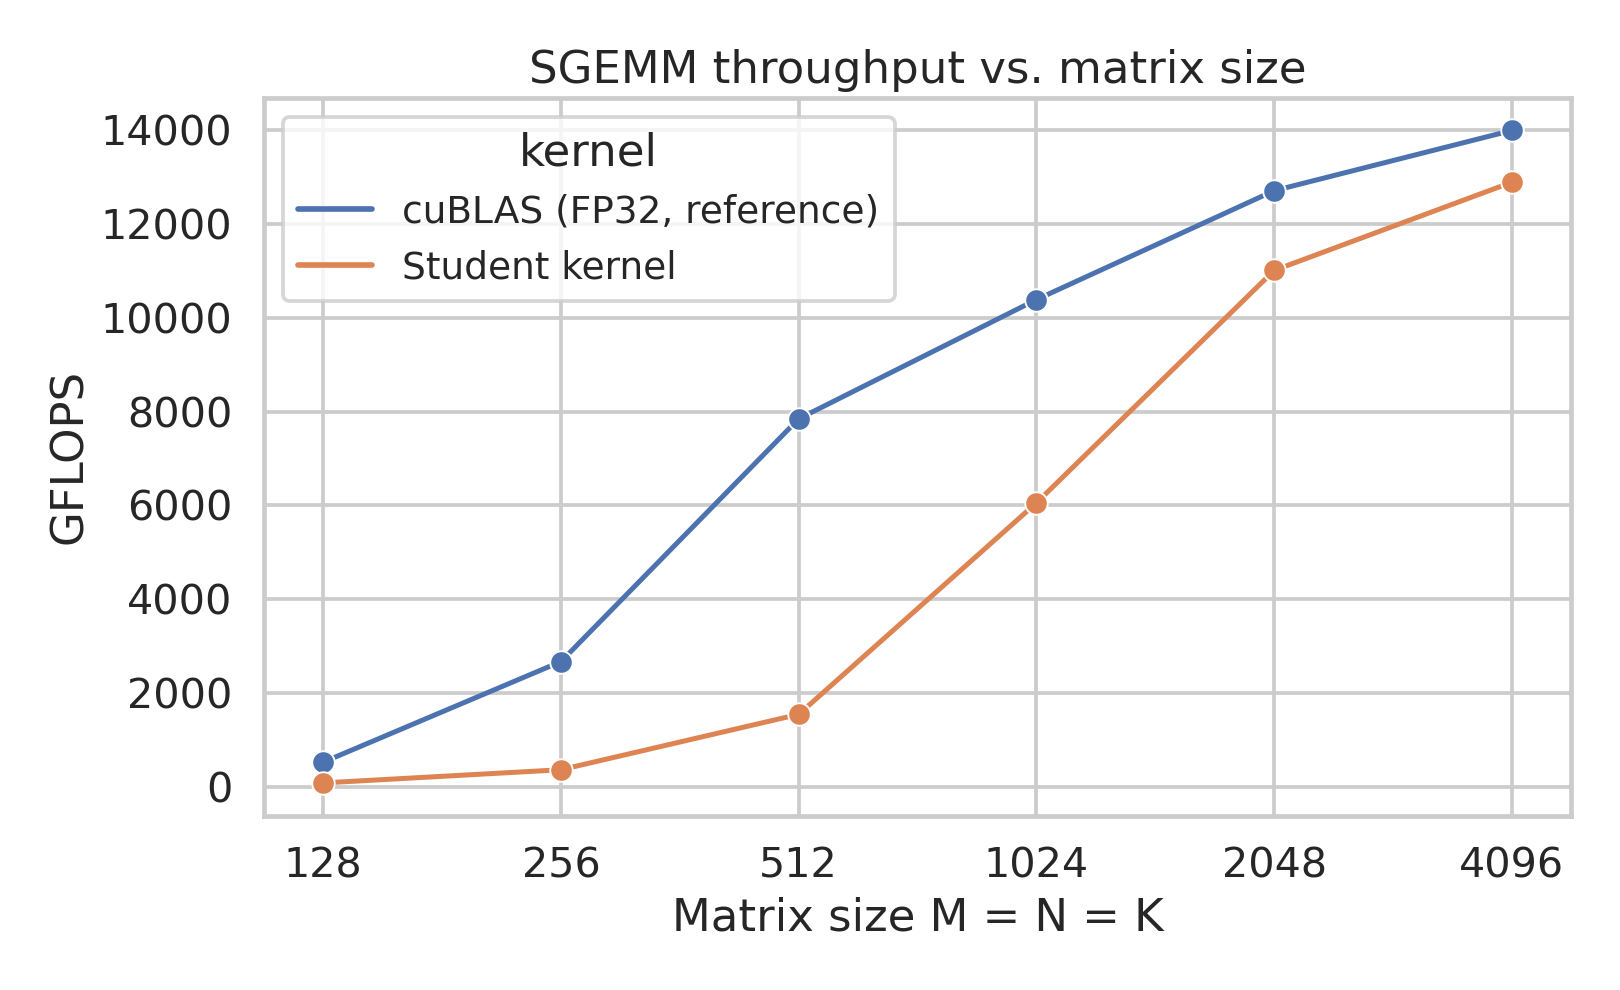
\includegraphics[width=0.82\linewidth]{figure/gflops_vs_size.png}
\caption{Student kernel vs.\ cuBLAS FP32 throughput across matrix sizes on TITAN RTX.}
\label{fig:scaling}
\end{figure}

\end{document}
